Data integration constitutes the issue of combining data residing at different sources and providing the user with a unified view of these data \cite{Lenzerini:2002:DIT:543613.543644}. 

We have now a definition of the concept data integration, but for what do we need it? The goal of data integration is almost always to simplify the access to a range of existing information systems through a central, integrated component with a unified interface for users and applications. Therefore, integrated information systems provide a unified view on the datasources. Existing datasources can be diverse: Classical relational database systems, files, data accessed by web services or HTML formulas, data generating applications or even other integrated information systems \cite[p. 3-4]{DBLP:books/dp/LeserN2006}.

In general, there are two different types of data integration: The \emph{materialized} integration and the \emph{virtual} integration. The difference between these two approaches reads as follows:

\begin{itemize}
 \item \label{materialized_index}in case of \emph{materialized} integration the data to be integrated is stored  into the integrated system itself. The data in the datasources remain, but for querying is used the materialized view. A classic example of a materialized data integration system are data warehouses.
 \item \label{virtual_index}in case of \emph{virtual} integration, the data are transported from the data source to the integrated system while the query processing. That temporary data is then again discarded. So, integration isn't done once but on each query.
\end{itemize}

Of course, an integrated information system can use both principles. A system of this kind is called \emph{hybrid}\label{hybrid_index}. Both types have in common that a query is processed on a global schema. For the virtual integrated system, the data only exists virtually, thus relations between data sources and the global schema have to be specified. Then, on query time the query has to be split into query schedules. The schedules are responsible for extracting the needed information from the different data sources and subsequently merge and transform the data \cite[p. 86-88]{DBLP:books/dp/LeserN2006}.


Today, data is classified into three diverse categories:
\begin{longtable}{|l|p{0.6\textwidth}|}
 \hline
 \textbf{Structured data}  &  Have a predefined structure through a schema.\\ \hline
 \textbf{Unstructured data}    &  Contains no predefined structure.\\ \hline
 \textbf{Semi-structured data} & This kind of data can also have a schema, but can deviate from the schema, too.\\ \hline
\caption{Types of data \cite[p. 17]{DBLP:books/dp/LeserN2006}}
\label{type_of_data_label}
\end{longtable}

A common example for structured data are relational data. Unstructured data can be seen as the opposite of structured data. Typical unstructured data is natural language text. Semi-structured data are in the middle between the other two, i.e. semi-structured data have structured data, but aren't forced to use a schema. An example of semi-structured data is an XML file without an accompanying XML schema.

A significant property to consider when looking at data is heterogeneity. What heterogeneity is and how it affects data integration will be explained in the next section. But before we explain it, we should introduce Some important terms and concept that we need to understand data integration and heterogeneity:

\textbf{Data model}: \label{data_model_index} In data modeling theory a data model is an abstract model that describes how data is represented and used. It consists of a set of data structures and conceptual tools that is used to describe the structure of a database and operations that can be performed on the data. A data model consists of a data model theory, a formal description of the data model, and a data model instance, which is a practical data model designed for a particular application. There exist three types of data models \cite[p.10-14]{IntroductionToDatabaseSystems2010}:
\begin{itemize}
	\item \textbf{Conceptual data model}: Describes data independent from any implementation details. It is used to describe the semantic of a domain. Examples for conceptual data models are the entity-relationship (E-R) model and ontologies. 
	\item \textbf{Logical data model}: Also called representational or implementation data model. Describes data in terms of data structures, like relational tables and columns or XML tags. Examples of logical data models are the relational data model, the object-based data model, semi-structured data models like XML or a graph-based data model like RDF. 
	\item \textbf{Physical data model}: Describes data in terms of collection of files, indices and other physical storage structures. It defines how the data is stored on disk and the available access methods. 
\end{itemize}

\textbf{Data source}:\label{data_source_index} A data source addresses an arbitrary data storage, whose data should be integrated in an information system \cite[p. 7]{DBLP:books/dp/LeserN2006}.

\textbf{Integrated or integrating information system}:\label{integrated_system_index} An integrated information system is an application, which facilitates the access to different data sources \cite[p. 7]{DBLP:books/dp/LeserN2006}.

\textbf{Meta data}:\label{meta_data_index} Data that describe other data. The distinction between data and meta data in a system depends on the particular application. Meta data has to be stored, browsed and integrated as well as 'normal' data \cite[p. 8]{DBLP:books/dp/LeserN2006}.

\textbf{Schema}:\label{schema_index} The word comes from greek \foreignlanguage{greek}{\emph{σχήμα}} (skhēma) meaning \emph{shape} or \emph{plan}. In computer science this word has different meanings. 
In the context of database theory the word is used for a representation of the structure (syntax), semantics, and constraints on the use of a database (or its portion) in a particular data model. \cite[p. 235]{Sheth:1990:FDS:96602.96604}. Analogous, an XML schema defines the structure, content and semantics of XML documents\cite{w3XMLSchema}. To generalize it, we can define a schema in the context of data integration as the definition of the structure, content and semantics of a data source.

\section{Heterogeneity}

Information systems providing not the same methods, models and structures for accessing their data are called \textit{heterogeneous} \cite[p. 58]{DBLP:books/dp/LeserN2006}. It commonly occurs that distributed systems (and therefore are maintained independently) tend to be heterogeneous, since they are managed autonomously. In other words, distribution often leads to heterogeneity, but not necessarily. De facto, it is to observe, that data sources tend to be the more heterogeneous the more autonomous they are. Two independent systems will in practice always  be heterogeneous, even if they contain the same kind of data. Heterogeneity arises from different requirements, different developers and different temporal developments. It even occurs if initially identical software systems are used, but over time they were adapted to the specific enterprise's needs. This process is called \textit{customizing}  \cite[p. 59]{DBLP:books/dp/LeserN2006}. 

Heterogeneity is the main issue of data integration \cite[p. 59]{DBLP:books/dp/LeserN2006}. As a consequence, integrated systems often restrict autonomy of the data sources making them more homogeneous. A common example would be the use of industry-specific standards like common exchange formats, interfaces or communication protocols.

Heterogeneity exists between the data sources, as well between the data sources and the integrated system \cite[p. 60]{DBLP:books/dp/LeserN2006}. But often only the latter case is relevant, as the data sources often don't communicate among themselves. To bridge heterogeneity, it obviously is necessary to translate queries and to implement missing functionality in the integrated system. An example of heterogeneity between a data source and the integrated system is, if the data source provides SQL-access, but the integrated system uses SPARQL for querying.

Heterogeneity is an issue we have to overcome in the thesis' project. It is necessary to have a thorough understanding of the nature of heterogeneity in order to overcome it correctly. Thus, we will discuss heterogeneity more in depth in the next sections. Heterogeneity can be split into different types: Table \ref{kinds-of-heterogeneity} shows an overview of the existing kinds of heterogeneity \cite[p. 60/61]{DBLP:books/dp/LeserN2006}.

\begin{longtable}{|l|p{0.6\textwidth}|}
%\centering
\hline
 \textbf{Technical  heterogeneity}  &  Includes all technical problems to realize the access of the data from the datasources.\\ \hline
 \textbf{Syntactic  heterogeneity}    &  Includes problems in the presentation of data.\\ \hline
 \textbf{Data model  heterogeneity} &  means problems in the presentation of data of the used data models. \\ \hline
 \textbf{Structural  heterogeneity}    &  Includes differences in the structural representation of information. This heterogeneity is solved if semantic identical concepts are also structural equally modeled. \\ \hline
 \textbf{Schematic  heterogeneity} &  Important special case of the structural heterogeneity, whereby there are differences in the used data model.\\ \hline
 \textbf{Semantic  heterogeneity}    &  Includes problems regarding the meaning of used terms and concepts.\\ \hline
\caption{Kinds of heterogeneity \cite[p. 60/61]{DBLP:books/dp/LeserN2006}}
\label{kinds-of-heterogeneity}
\end{longtable}

\subsection{Technical  heterogeneity}
This kind of heterogeneity defines differences between information systems to access their data. There are different technical layers on which heterogeneity can exist \cite[p. 62]{DBLP:books/dp/LeserN2006}:
\begin{itemize}
\item \textbf{Request function:} query language, parameterized  functions, canned queries (forms)
\item \textbf{Query language:} SQL, XQuery, SPARQL, full text search
\item \textbf{Exchange format:} binary data, XML, HTML, tabular
\item \textbf{communication protocol:} HTTP, JDBC, SOAP
\end{itemize}

Technical heterogeneity can be further subdivided in \cite[p. 64]{DBLP:books/dp/LeserN2006}: \label{technical_heterogeneity_subtypes}
\begin{itemize}
\item \textbf{Access heterogeneity:} Authentication and authorization differences between information systems
\item \textbf{Interface heterogeneity:} Differences in the technical realization of data source access. A special case here is heterogeneity in the query mechanism, e.g. the used query language.
\end{itemize}

Technical  heterogeneity is overcome if the integrated system is able to send a query to a data source and that data source principally understands the query and produces a set of data as a result \cite[p. 61]{DBLP:books/dp/LeserN2006}.

\subsection{Syntactic  heterogeneity}
Syntactic heterogeneity describes differences in the presentation of the same facts\cite[p. 64]{DBLP:books/dp/LeserN2006}. For example, different number formats (little endian and big endian), different character encodings (Unicode, ASCII) or different separators in text files (tab delimited and comma separated values (CSV)). Syntactic heterogeneity therefore can be reduced to technical differences in the presentation of information, whereas the \textit{synonym problem,} which deals with the representation of equal concepts through different names, is an issue of \textit{semantic heterogeneity}.

This kind of heterogeneity is overcome if all data meaning the same are presented equally \cite[p. 61]{DBLP:books/dp/LeserN2006}.

\subsection{Data model  heterogeneity}
Data model heterogeneity arises if the integrated system and a data source manage their data in different data models \cite[p. 65]{DBLP:books/dp/LeserN2006}. Data model usually means the \emph{conceptual} or the \emph{logical} data model (or both), as the physical data model is only used for internal processing inside the data source and never propagated outwards.

Important to note is the fact, that data model heterogeneity is independent from \emph{semantic} differences. Two systems can use two different data models both describing the same domain, e.g. describing data in the object oriented or relational data model. Nevertheless, it is to observe that differences in the data model often induces semantic heterogeneity.

Data model heterogeneity is solved if the data sources and the integrated system use the same data model \cite[p. 61]{DBLP:books/dp/LeserN2006}.

\subsection{Structural  heterogeneity}
Using the same data model doesn't mean semantic equal data has to be described equally. We speak of structural heterogeneity if two schemas are different, even though they represent the same extract of the real world (i.d. the intension of their schema elements is equal) \cite[p. 67]{DBLP:books/dp/LeserN2006}. 

Structural heterogeneity can have many reasons like different preferences of developers, different requirements, using different data models, technical restrictions, etc. . This arises from the \textit{design autonomity} of data sources. A Data source has design autonomity if it can freely decide in which way it provides its data, including the data format, the data model, the schema, syntactic represenation of data, the use of concept systems, and the units of values \cite[p.55]{DBLP:books/dp/LeserN2006}.

This heterogeneity is solved if semantic identical concepts are also structural equally modeled  \cite[p. 61]{DBLP:books/dp/LeserN2006}.

\subsection{Schematic  heterogeneity}
A special case of structural heterogeneity is schematic heterogeneity \cite[p. 67]{DBLP:books/dp/LeserN2006}. Schematic heterogeneity is present if different elements of the data model are used to model the same thing. In the relational model it is possible to model information as relations, as attributes or as values, for instance. 

Schematic conflicts are particularly difficult to resolve, as it isn't usually possible to overcome them with the query language \cite[p. 68]{DBLP:books/dp/LeserN2006}. For example, it is mandatory to explicitly state attributes and relations in relational languages. If schematic heterogeneous data sources should be integrated, one would define a view. But the query has to be altered if something changes in the elements.

\subsection{Semantic  heterogeneity}
Individual values have no implicit meaning in an information system. Looking at the number '20' on a table doesn't allow conclusions concerning its meaning. In fact, it could be anything. Only by \textit{interpreting} a datum it gets a meaning, and for interpretation one needs knowledge about the concrete use case and world knowledge. The interpretation of data is also called \textit{semantic}. Therefore, to interpret data in an information system, further information has to be consulted \cite[p. 73]{DBLP:books/dp/LeserN2006}:
\begin{itemize}
\item The name of the schema element containing the data
\item The position of the schema element within the schema
\item Knowledge about the domain the schema is developed for.
\item Other data values stored in the schema element
\end{itemize}

Comprehending all this information, we speak of the data's \textit{context} \cite[p. 74]{DBLP:books/dp/LeserN2006}. 
Data only obtain its meaning by taking its context into account. But it should be considered that some parts of the context are given in machine-readable form (like the schema), and some are not (e.g. domain specific knowledge). 
Also absolutely identical schemas with different contexts can have different semantic meanings. Owing to circumstances, an integrated system has to make implicit context knowledge explicit, e.g. by introducing new schema elements.

Semantic conflicts relate to the interpretation of \emph{names} and \emph{symbols}, respectively \cite[p. 74]{DBLP:books/dp/LeserN2006}. 
Semantic conflicts occur in the interaction of names and concepts in different systems. 
In this context, a \textit{concept} means the intension of a name. The set of real world objects of a name is called its \emph{extension}. 
The most common semantic conflicts are synonyms and homonyms \cite[p. 75]{DBLP:books/dp/LeserN2006}. 
Two names are \textit{synonyms} if they have the same intension, but are syntactic different. An example of synonyms are the words \emph{disease} and \emph{illness}. They mean the same but are different words.

Whereas two names are \textit{homonyms} if they are syntactically identical, but their intensions are different. Example: Two tables contain a column called \emph{date}. The first table stores dates about the beginning of a treatment whereas the other table stores dates of births.

More difficult to treat are names, though, whose intensions neither are identical nor completely different, but conclude themselves or are overlapping.
Example: We have two names \emph{patient} and \emph{person}. Not every person is automatically a patient and also a patient needn't to be also a person (e.g. an animal could be a patient in the veterinary medicine). But in certain contexts, \emph{patient} and \emph{person} can be seen to be equal.

In principle, it is difficult to detect semantic conflicts and resolve them clearly \cite[p. 76]{DBLP:books/dp/LeserN2006}. 
It has to be considered that often for schema analysis  only the schema is available and some example data, sometimes maybe also some domain knowledge and documentation of the data sources, but that isn’t always the case, particularly on autonomous systems. Especially difficult are cases with less clear defined concepts or with options for multiple interpretations.

A complete resolving of semantic conflicts isn't always possible, or only achievable with big effort, or not necessary. This is also called \textit{remaining blur} \cite[p. 76]{DBLP:books/dp/LeserN2006}.

Semantic heterogeneity is solved if the integrated system and the data source really mean the same by the used names for schema elements. Equal names have consequently equal meaning \cite[p. 61]{DBLP:books/dp/LeserN2006}.

\section{Distribution}

An issue of data integration is the distribution of data to be integrated \cite[p. 51]{DBLP:books/dp/LeserN2006}. We speak thereby of data which lies on different systems. 
Important to know, we proceed the assumption that the acccess to the data is ensured, i.e. the systems are connected.

Data distribution isn't plainly an annoyance, as it is often an intended design decision\cite[p. 54]{DBLP:books/dp/LeserN2006}. The distribution is handy for load balancing, reliability and protection against data loss. Thereby the distribution is controlled on a central point. 
The consistency of data is assured using sophisticated mechanisms like the 2-phase-commit protocol\cite[p. 54]{DBLP:books/dp/LeserN2006}. Contrary, in a typical data integration project distribution of data has historically evolved or is due to organizations and thus is uncontrolled redundant.

Distribution can be structured into logical and physical distribution \cite[p. 51]{DBLP:books/dp/LeserN2006}. Data is \textit{physical} distributed if it lies onto physical different systems
which geographically also can be located on different places. In turn, data is \textit{logical} distributed, if there exists multiple possible locations for storing the same data. 

\subsection{Physical distribution}
In order to integrate physical distributed data several issues have to be solved \cite[p. 51]{DBLP:books/dp/LeserN2006}: the first step is to detect the physical storage location of the data. Therefore, computer, server, port, and network have to be identifiable and locatable. For identification, applications used in the internet use Uniform Resource Locators (URLs) to identify remote computers and services not knowing their exact location.

The second problem resulting from physical distribution is data stored in different schemas \cite[p. 52]{DBLP:books/dp/LeserN2006}. However, common query languages don't provide the possibility to query data residing in different schemas. There are two different solutions:
\begin{itemize}
\item Separating a query into several schema specific queries and consolidating the results in the integrated system.
\item Developing a language able to handle several schemas in a posed query.
\end{itemize}

Physical distribution also changes the requirements for the query optimizer \cite[p. 52]{DBLP:books/dp/LeserN2006}: In a central database the optimizer's main function is minimizing  the accesses to the local storage, whereas for a distributed database the accesses over the network should be held as small as possible. This is important as remote accesses need considerably more time than accesses to the local storage.  

\subsection{Logical distribution}
If identical data is located on different locations inside the same system, we speak of a logical distribution \cite[p. 52]{DBLP:books/dp/LeserN2006}. The key property of logical distribution is therefore the \textit{overlapping of the intension} of different data storage locations. Thereby, it is insignificant where these systems physically really are. Two database instances on one computer induce already distribution issues.

In this context redundany plays a major role in a system \cite[p. 53]{DBLP:books/dp/LeserN2006}. A distributed system is called redundant if semantically identical data can be located at different places. In order to get a consistent view of a redundant system, redundancy has to be strictly controlled (e.g. using triggers or replication mechanisms). At anytime it has to be assured that the same data is at all different places. 
But data integration typically has to deal with \textit{uncontrolled redundancy} for each data source is maintained independently. This fact leads to several problems \cite[p. 53]{DBLP:books/dp/LeserN2006}:

\begin{itemize}
\item \textbf{Localization}: The integrated system has to provide meta data allowing to \textit{locate} data. E.g. this can be done by a catalog of all schemas and their descriptions or a global schema with mappings to source schemas.
\item \textbf{Duplicates}: If it is possible that data exists on multiple locations, there will exist duplicates, i.e. objects stored on both locations. These objects have to be recognized by the integrated system.
\item \textbf{Inconsistencies}: Redundant data can contain inconsistencies that have to be resolved for a homogeneous presentation.
\end{itemize}

\section{Architectures}

In order to design a system for a data integration process, it is necessary to understand the basic architectures that we found for data integration, so that a suitable reference architecture can be chosen. For this, we will different architectures in the following.
%we will look at different architectures in the following. 

%In the following basic database concepts, on which integrated systems base, are explained. Additionally different types of integrated systems are presented shortly.

Integrated systems evolved from distributed databases which in turn are based on the classical \emph{monolithic database}. 
This system is subdivided into three layers as shown in figure \ref{MonolithicDatabaseArchitecture} and is based on the ANSI/X3/SPARC three-layer architecture \cite{TSICHRITZIS1978173}, \cite[p. 84/85]{DBLP:books/dp/LeserN2006}.

The \textit{internal (or physical) view} is responsible for the storage of the data on the respective database. 
One layer upwards comes the \textit{conceptual (or logical) view} modeling the data on a conceptual way. The conceptual schema defines which data model is used, which data is stored in the DBMS, and the relations among the data.
Splitting the data into the internal and conceptual view makes the data independent from the physical storage medium. The top layer is called \textit{external (or export) view} and is responsible with modeling of data as well as the conceptual view. However, it isn't modeled the whole application domain. The external view only specifies which part of the conceptual schema is provided to the respective application. An export schema is initially a subset of the conceptual schema, but can be transformed and aggregated. In the external view are defined access restrictions, too. Splitting up conceptual and external view ensures \textit{logical data independence}.

\begin{figure}[H]
	\begin{center}
		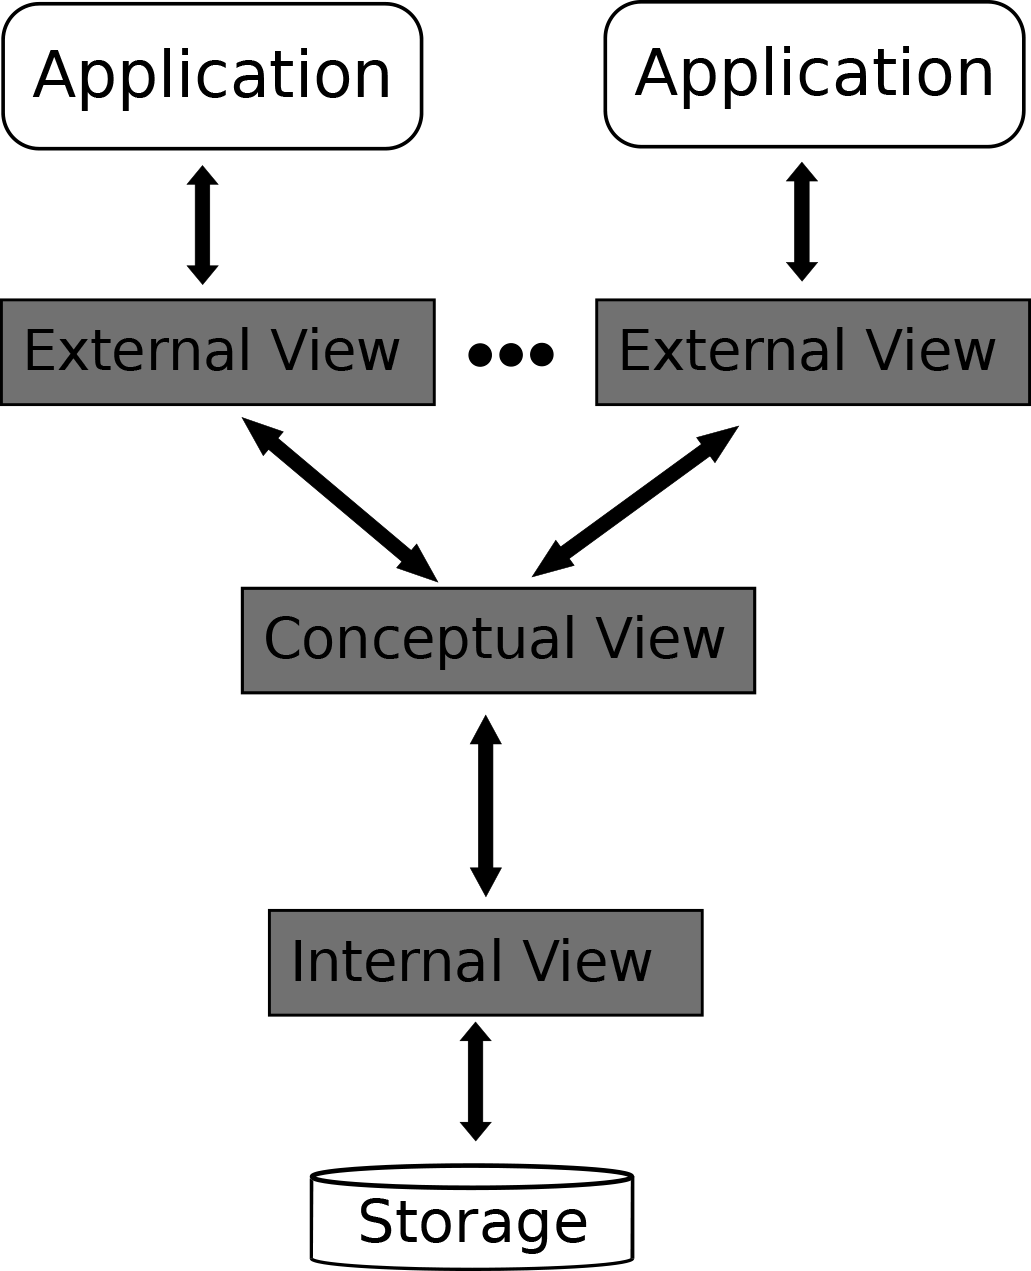
\includegraphics[scale=0.5]{figures/monolithicalDatabaseArchitecture.png}
	\end{center}
	\caption{ANSI/X3/SPARC three-layer architecture \cite[p. 85]{DBLP:books/dp/LeserN2006}}
	\label{MonolithicDatabaseArchitecture}
\end{figure} 


\subsection{Distributed Systems}

From the monolothic database evolved the distributed database architecture, as shown in figure \ref{DistributedDatabaseArchitecture}.

\begin{figure}[H]
	\begin{center}
		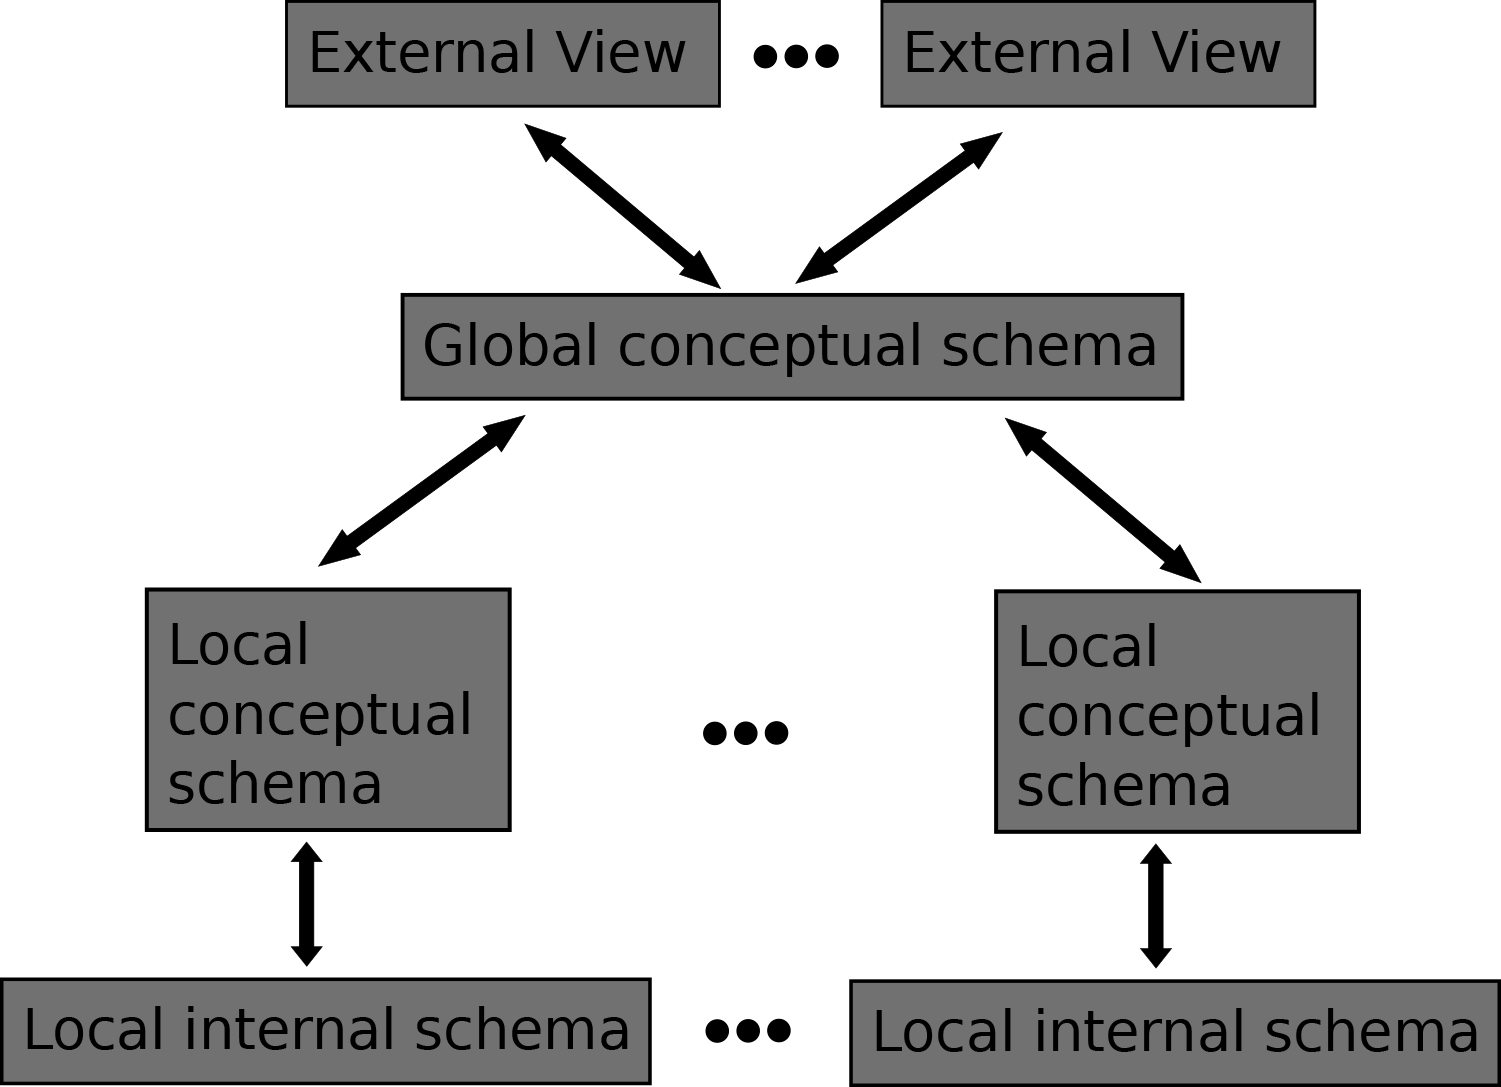
\includegraphics[scale=0.5]{figures/distributedDatabaseArchitecture.png}
	\end{center}
	\caption{Architecture of a distributed database \cite[p. 92]{DBLP:books/dp/LeserN2006}}
	\label{DistributedDatabaseArchitecture}
\end{figure}


The idea with distributed systems is to distribute data onto several systems (physical and logical), but it should be possible to query all data at once. In order to achieve this, the architecture is subdivided into \textit{four layers}. Each datasource has a local internal and local conceptual schema. The latter only mirrors the data managed by the local database. Dependent on the used distribution strategy, the local conceptual schema is equal to the global conceptual schema  or an extract from it. Common distribution strategies are vertical and horizontal partitioning \cite[p. 92]{DBLP:books/dp/LeserN2006}: 
\begin{itemize}
\item \textbf{horizontal partitioning:} Data of big tables is distributed per tuples on different computers. A union operation consolidates these parts again.
\item \textbf{vertical partitioning:} Data of big tables is distributed per attributes on different computers. Each partition contains additionally a shared key attribute. This makes it possible to consolidate the partitions with a join operation.
\end{itemize}
On top of the local conceptual schemes stands a global conceptual schema. This schema models the whole application domain and is the central point of reference for the external schemes playing the same role as in the three-layers-architecture.

Distributed databases are close coupled. They are strictly controlled while conception and operation and thus the main problems of heterogeneity (like structural and semantic heterogeneity) don't occur \cite[p. 93]{DBLP:books/dp/LeserN2006}. 
Thus, this architecture is good for environments, there the datasources to be distributed are less heterogeneous. For highly heterogeneous systems (like medical datasources), though, this architecture is unsuitable.
 

\subsection{Multidatabase Systems}

For to enable heterogeneous databases to connect, the Multidatabase System (MBS) architecture has been evolved (shown in figure \ref{MBSDatabaseArchitecture}). 

\begin{figure}[H]
	\begin{center}
		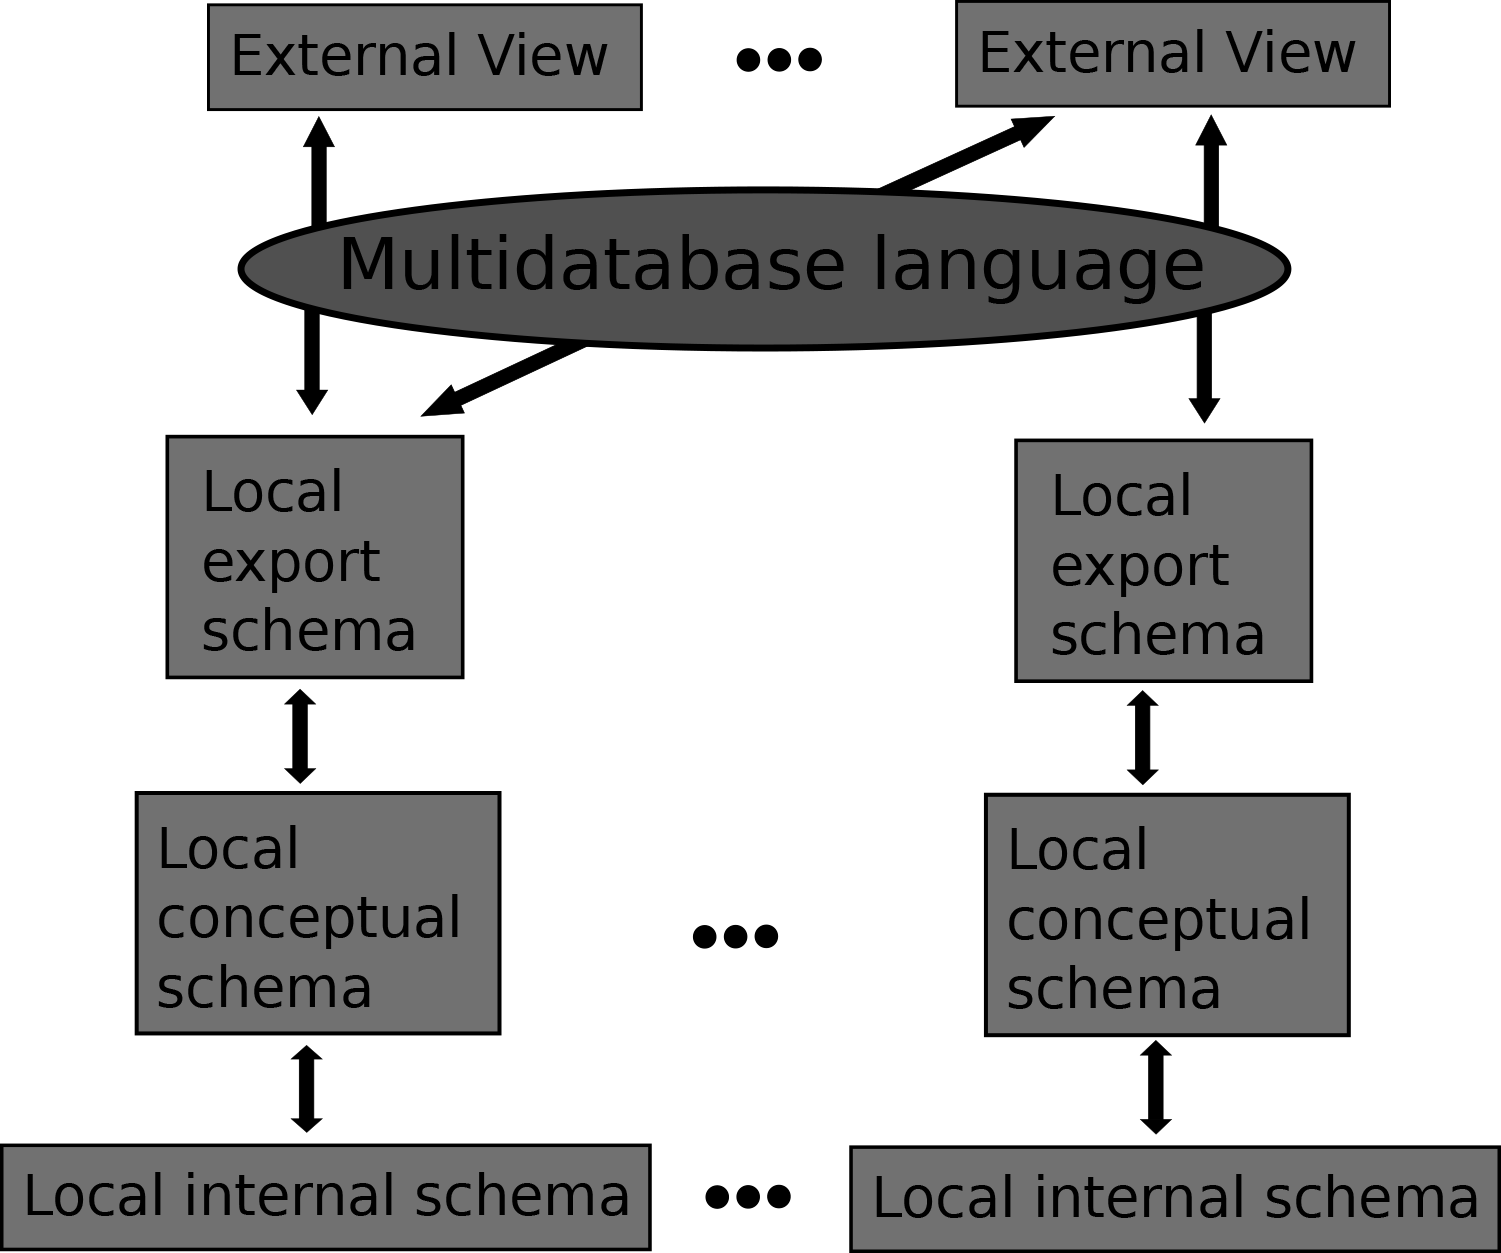
\includegraphics[scale=0.5]{figures/MultidatabaseArchitecture.png}
	\end{center}
	\caption{Architecture of a  multidatabase system \cite[p. 94]{DBLP:books/dp/LeserN2006}}
	\label{MBSDatabaseArchitecture}
\end{figure}

MBSs are collections of autonomous databases being loosely linked \cite[p. 93]{DBLP:books/dp/LeserN2006}. Each database grants external applications access to its data. The access is done using a database language which allows to query several databases in one query. 
A language of that kind is called multidatabase language. To obtain the autonomy  of the involved databases, a MBS has no global conceptual schema. Instead, each local database keeps an export schema defining which part of the local conceptual schema is provided to external applications.  
It is assumed that no data model heterogeneity is contained in a MBS, i.e. all databases use the same data model, or either the multidatabase language or the local datasource provide a translation to the global data model. Now, each application can create its own external schema, which integrates one or more data sources. So, it's the task of the application doing the integration task. A MBS provides only a suitable language for querying \cite[p. 94]{DBLP:books/dp/LeserN2006}.	
It can be noted that a MBS is only suitable for datasources that use the same data model. If this is not the case, another system has to be used. Furthermore should be considered: the query language has to support all languages of the data sources. In order to add a datasource with a not supported query language the MBS query language has to be altered. 

\subsection{Federated Systems}

In contrast to MBSs, federated database management systems (FDBMS) have a global conceptual schema as seen in figure \ref{FDBMSArchitecture}. The schema is also called the \emph{federated schema}.

\begin{figure}[H]
	\begin{center}
		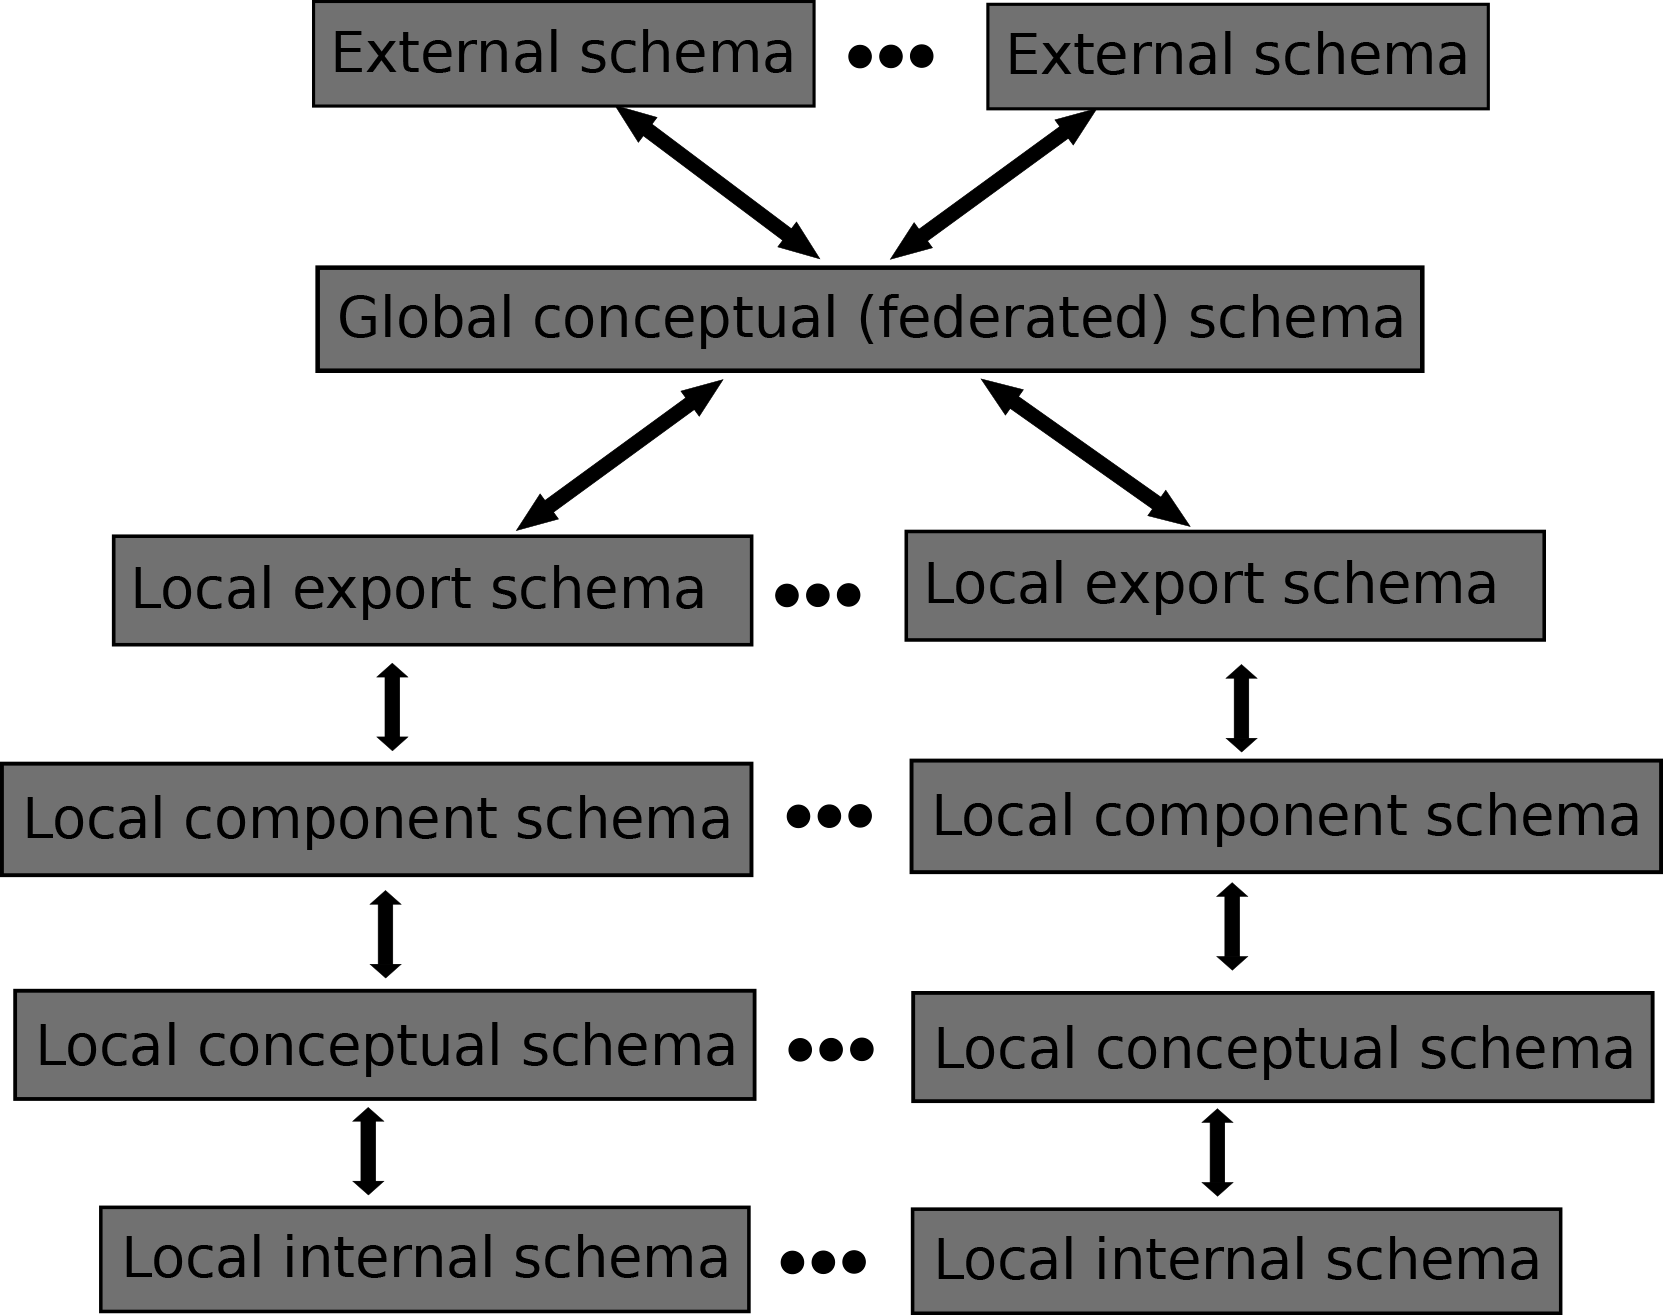
\includegraphics[scale=0.5]{figures/federatedDatabaseArchitecture.png}
	\end{center}
	\caption{Architecture of a  federated database management systems (FDBMS) \cite[p. 95]{DBLP:books/dp/LeserN2006}}
	\label{FDBMSArchitecture}
\end{figure}

The federated schema is the central point of reference for all external schemes and there applications \cite[p. 94]{DBLP:books/dp/LeserN2006}. But in contrast to distributed databases the global schema results after the local schemes with the goal to provide an integrated view of existing and heterogeneous data sets. Data sources keep a high degree of autonomy. The used data model in the global scheme is known as the \emph{canonical} data model. 

All in all, a FDBMS consists of five different layers \cite[p. 95]{DBLP:books/dp/LeserN2006}:

\begin{itemize}
\item \textbf{Local conceptual schema}: Defines the data of a data source. Is comparable with the conceptual schema of the three-layer architecture.
\item \textbf{Local component schema}: Defines the data of the local conceptual schema in the canonical data model. 
\item \textbf{Local export schema}: Does the same as the external view in the three-layer architecture, it defines which elements of the local component schema are visible/query-able from the outside.
\item \textbf{Global conceptual/federated schema}: Defines an integrated view over all data sources and is defined in the canonical data model. The federated schema consists of multiple export schemas \cite[p. 200]{Sheth:1990:FDS:96602.96604}.
\item \textbf{External schema}: Defines a subset of the global schema that should be visible to an application.
\end{itemize}

Remarkable is, a federal system can have several federated schemas that integrate differently the export schemas. This allows data with different semantic meaning within the federated system when combining query results of different federated schemas. But query results of a specific federated schema are always semantically integrated, so, there is no data co-existence between them. As we will see later, this is a crucial difference in respect to dataspaces.

\subsection{Mediator-based Systems}

Mediator-based information systems are a generalization of the previous architectures (see figure \ref{MediatorBasedArchitecture}) \cite[p. 97]{DBLP:books/dp/LeserN2006}: They know only two separate components, namely Wrappers and Mediators. 

\begin{figure}[H]
	\begin{center}
		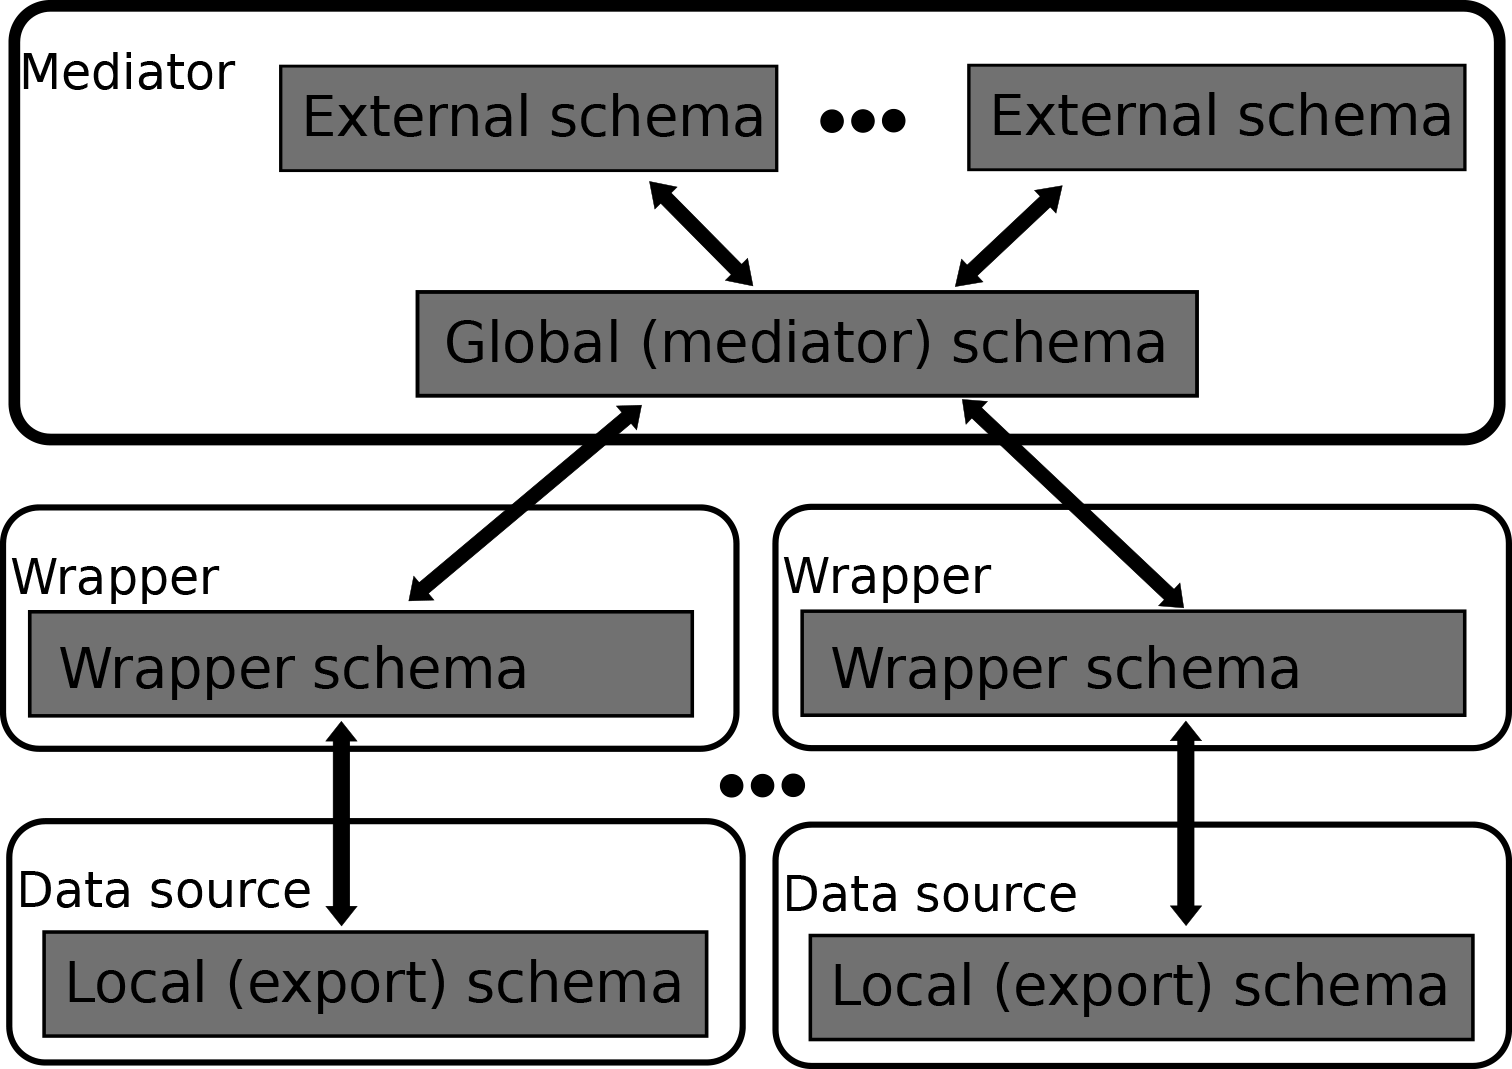
\includegraphics[scale=0.5]{figures/MediatorBasedArchitecture.png}
	\end{center}
	\caption{Architecture of a  mediator-based information system \cite[p. 97]{DBLP:books/dp/LeserN2006}}
	\label{MediatorBasedArchitecture}
\end{figure}

Wrappers are software components responsible for the access to a solely data source.
A Wrapper has to break down technical, data model, schematic and interface (technical) heterogeneity. It realizes the communication between the mediators and datasources, and includes following tasks:

\begin{itemize}
\item overcoming interface heterogeneity (e.g. SQL to html formulars)
\item overcoming language heterogeneity. This includes the handling of restricted data sources and different query languages.
\item providing data model transparency through translating the data into the canonical data model.
\item resolving schema heterogeneity by using a suitable mapping between the source schema and the global schema.
\item supporting the global query optimizing by providing information about the query capabilities of the data source and expected costs.
\end{itemize}

The thesis' system project uses wrappers. Thus we go more in depth and look at the design, architecture and implementation goals of an architecture using wrappers. The following statements are results of from \cite{Roth:1997:DSW:645923.670992}:

\textbf{Low start-up costs:} Writing a wrapper should be done very quickly, very simple wrappers even within a few hours. The authoring of a wrapper should also be as simple as possible for writing the wrapper with little or no knowledge about the internal structure of the integrated system.

\textbf{Easy evolving:} Evolving should be done very simple due to two reasons: a wrapper should be implemented very fast to show feasibility. More sophisticated features a datasource can provide should be added later. Additionally the data source can change itself over time and the wrapper should be easily adaptable. 


The second component of a mediator-based ssystem is the mediator software component which uses knowledge of certain data to \textit{create and provide} information for other applications. Mediators communicate with one or more wrappers and deliver a specific value, normally structural and semantic data integration.

The following list shows an extract of the services a mediator might provide (from, \cite[p. 5-6]{Wiederhold1996TheCB}): 
\begin{itemize}
\item Selection of likely relevant data, e.g. used for scoring query results
\item Invocation of wrappers to deal with legacy sources
\item Resolution of domain term	terminology and ontology differences
\item Sending data and meta-data to the customer application
\item Imposition of security filters to guard private data
\item Handling data duplication, e.g. by deleting it
%\item Assessment of quality of the data from the data sources
\item Integration of data from several data sources
\end{itemize}

In a mediator-based architecture data sources don't know of the existence of the integrated system: only the wrapper directly speaks with the data source. As a result autonomy is preserved for all data sources \cite[p. 97]{DBLP:books/dp/LeserN2006}.


%In \textbf{peer data management systems} (PDMS) there is no separation between data source and integration system. Query can be posed from every system to every other system within the integrated system. The other system than tries to calculate responses with own or other sourced data. So each participant of the integrated system, a so-called peer, is a mediator and a data source at the same time.  

\section{Ontologies}

In computer science an ontology defines the concepts, relationships, and other distinctions being relevant for modeling a domain \cite{9780387355443}. It operates on the semantic level and thus is independent from lower data models (logical and physical data models). Since ontologies are independent from lower level data models, they are suitable for integrating heterogeneous data sources. Data integration using ontologies is also called \emph{ontology-based} integration.

To specify an ontology description logics are used \cite[p. 267]{DBLP:books/dp/LeserN2006}. With description logics it is possible to define classes of a domain and the relations between these classes. An advantage is that by using description logics a domain can be specified much more precisely than using the relational data model. 

Ontologies can generate new knowledge from existing data by using \emph{logical inference}: The ontology defines basic rules in a formal model, and by applying these rules on a given data set the ontology might infer knowledge from it that wasn't explicitly stated before.